\chapter{Safety-Critical Java Virtual Machine Services}
\label{scjvm-services-chapter}

In order to reason about a Safety-Critical Java virtual machine
(SCJVM), we first require an identification of the the requirements of
an SCJVM and a formal model of those requirements.
For the purposes of our model, we consider an SCJVM to have the
components illustrated in Figure~\ref{scjvm-services-fig}.
An SCJVM is divided into two main parts:~the core execution
environment, and the SCJVM services, which may make use of the services
of an underlying operating system or hardware abstraction layer.

\begin{figure}[ht]
  \centering
  \begin{tikzpicture}

    \coordinate (width)  at (10cm,0cm);
    \coordinate (height) at (0cm,7cm);

    \path (0,0) -- (height)
    coordinate[pos=0.18] (OS boundary)
    coordinate[pos=0.20] (VM part bottom)
    coordinate[pos=0.57] (VM part top)
    coordinate[pos=0.60] (API boundary)
    coordinate[pos=0.82] (App boundary);
    
    \path (VM part bottom) -- (VM part top)
    coordinate[pos=0.7] (VM Service top);

    \path (VM part bottom) -- (VM part top)
    coordinate[pos=0.85] (VM Services ypos);

    \path (0,0) -- (width)
    coordinate[pos=0.04] (CEE left)
    coordinate[pos=0.27] (CEE right)
    coordinate[pos=0.29] (VM Services left)
    coordinate[pos=0.96] (VM Services right)
    coordinate[pos=0.17] (VM Service width)
    coordinate[pos=0.04] (VM Service sep);

    \path (VM Services left) -- (VM Services right)
    coordinate[pos=0.5] (VM Services xpos);

    \path (0,0) to node[pos=0.5] (mid) {} (width);
    \path (0,0) to node[pos=0.25] (quart) {} (width);

    \draw (0,0) rectangle (width |- height);

    \draw (OS boundary) -- ++(width);
    \path (0,0) rectangle node[pos=0.5] (OS) {} (width |- OS boundary);
    \draw (mid |- API boundary) rectangle node[pos=0.5] (API) {} (width |- App boundary);
    \draw (App boundary) -- ++(width);
    \path (App boundary) rectangle node[pos=0.5] (App) {} (width |- height);

    \path (quart |- API boundary) rectangle node[pos=0.4] (SCJVM) {} (quart |- App boundary);
    \draw (CEE left |- VM part bottom) rectangle node[pos=0.5] (CEE) {} (CEE right |- VM part top);
    \draw (VM Services left |- VM part bottom) rectangle (VM Services right |- VM part top);
    \coordinate (VM Services) at (VM Services xpos |- VM Services ypos);

    \node[align=center] at (App)   {SCJ Application};
    \node[align=center] at (API)   {SCJ\\Infrastructure\\and API};
    \node[align=center] at (SCJVM) {SCJ\\Virtual Machine};
    \node[align=center] at (CEE)   {Core\\Execution\\Environment};
    \node[align=center] at (OS)    {Operating System/Hardware Abstraction Layer};
    
    \foreach \x in {1,...,3}
    \pgfmathsetmacro{\a}{0.333*(\x - 1)}
    \pgfmathsetmacro{\b}{0.333*\x}
    \path ($(VM Services left) + (VM part bottom)!0.07!(VM part top)$) -- 
    node[pos=\a] (VM Service \x start) {}
    node[pos=\b] (VM Service \x end) {}
    ($(VM Services right) + (VM part bottom)!0.07!(VM part top) - (VM Service sep)$);

    \foreach \x in {1,...,3} 
    \draw ($(VM Service \x start) + (VM Service sep)$)
    rectangle node[pos=0.5] (VM Service \x) {}
    (VM Service \x end |- VM Service top);

    \node[align=center] at (VM Services)  {VM Services};
    \node[align=center] at (VM Service 1) {Memory\\Manager};
    \node[align=center] at (VM Service 2) {Scheduler};
    \node[align=center] at (VM Service 3) {Real-time\\Clock};
  \end{tikzpicture}
  \caption{A diagram showing the structure of an SCJVM and its
    relation to the SCJ infrastructure and the operating
    system/hardware abstraction layer, focusing on the SCJVM services}
  \label{scjvm-services-fig}
\end{figure}

The core execution environment manages the execution of Java bytecode,
whether that be via interpretation, just-in-time compilation or
ahead-of-time compilation.
The core execution environment must also manage data that relates to
the execution of bytecode instructions, such as the representation of
classes and objects.

The SCJVM services represent the additional services that must be
offered by an SCJVM in order to support the SCJ infrastructure.
These services may be supplied as standalone services and so do not
need to be handled by the compilation strategy.
We consider the virtual machine services to be divided into three
areas:
\begin{itemize}
\item the memory manager, which manages backing stores for memory areas and
  allocation within them;
\item the scheduler, which manages threads and interrupts, and allows for
  implementation of SCJ event handlers; and
\item the real-time clock, which provides an interface to the system real-time
  clock.
\end{itemize}
Each of these services is used either by the core execution
environment or by the SCJ infrastructure.
Some of the services also rely on each other. 
For example, the real-time clock must communicate with the scheduler
to trigger an interrupt handler when an alarm's time passes.

A model of the core execution environment is presented in
Chapter~\ref{cee-chapter}.
In this chapter, we present the requirements for each area of the
SCJVM services:~the memory manager in
Section~\ref{memory-manager-section}, the scheduler in
Section~\ref{scheduler-section}, and the real-time clock in
Section~\ref{realtime-clock-section}.
The formal model of the SCJVM requirements is presented in
Section~\ref{formal-model-section}.
A complete version of the model can be found in
Appendix~\ref{full-scjvm-services-model}

The memory manager model has been subject to proof using Z/Eves.
The theorems proved about the memory manager can be found in
Appendix~\ref{memory-manager-theorems}, with the Z/Eves proof scripts
in Appendix~\ref{memory-manager-proofs}.
Many additional lemmas about objects in the Z/Eves mathematical
toolkit have been proved in the course of carrying out these proofs.
As these can be of use outside our work, we have included them
separately in Appendix~\ref{additional-lemmas} with their proofs in
Appendix~\ref{additional-lemmas-proofs}.

Part of an earlier version of this model was presented at the 13th
International Workshop on Java Technologies for Real-time and Embedded
Systems~\cite{baxter2015a} with the full earlier version made available
as a technical report~\cite{baxter2015}.

\section{Memory Manager API}
\label{memory-manager-section}

The SCJVM memory manager deals with the raw blocks of memory used as
backing stores for the memory areas of SCJ.
The memory areas themselves are Java objects, and so are dealt with by
the core execution environment and accessed through the SCJ API,
instead of directly via the virtual machine.
This is in line with what is specified in the SCJ standard and also
done for RTSJ.
Backing stores are assumed to have unique identifiers that can be used
to refer to them; these identifiers can be simply pointers to the
physical blocks of memory used for backing stores.

Each backing store is composed of two parts:~an area of memory in
which memory for objects may be allocated, and an area in which other
backing stores can be allocated.
A backing store may thus have other backing stores nested within it,
so that a possible memory layout is as shown in
Figure~\ref{memory-fig}.
There, we divide the two parts of each backing store by a dashed line,
with the object allocation area below and the backing store area
above.

\begin{figure*}[ht]
  \centering
  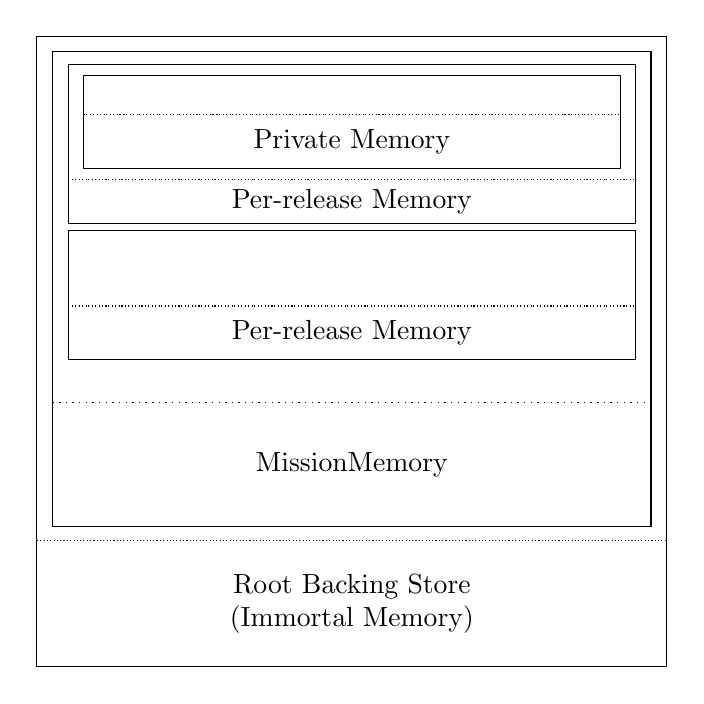
\begin{tikzpicture}

    \path (0,0) --
    node[pos=0.0] (RootBSLeft) {}
    node[pos=1.0] (RootBSRight) {}
    node[pos=1] (width) {}
    (8cm,0);

    \path (0,0) --
    node[pos=0.0] (RootBSBot) {}
    node[pos=0.2] (RootBSMid) {}
    node[pos=1.0] (RootBSTop) {}
    node[pos=1] (height) {}
    (0,8cm);

    \draw (RootBSLeft |- RootBSBot) rectangle (RootBSRight |- RootBSTop);
    \draw[dotted] (RootBSLeft |- RootBSMid) rectangle (RootBSRight |- RootBSMid);
    \path (RootBSLeft |- RootBSBot) rectangle (RootBSRight |- RootBSMid)
    node[pos=0.5,align=center] {Root Backing Store\\(Immortal Memory)};

    \path (RootBSLeft) --
    node[pos=0.01] (MisMemLeft) {}
    node[pos=0.99] (MisMemRight) {}
    (RootBSRight);

    \path (RootBSMid) --
    node[pos=0.01] (MisMemBot) {}
    node[pos=0.99] (MisMemTop) {}
    (RootBSTop);
    \path (MisMemBot) -- (MisMemTop) node[pos=0.25] (MisMemMid) {};

    \draw (MisMemLeft |- MisMemBot) rectangle (MisMemRight |- MisMemTop);
    \draw[dotted] (MisMemLeft |- MisMemMid) rectangle (MisMemRight |- MisMemMid);
    \path (MisMemLeft |- MisMemBot) rectangle (MisMemRight |- MisMemMid)
    node[pos=0.5,align=center] {MissionMemory};

    \path (MisMemLeft) --
    node[pos=0.01] (HdlrMemLeft) {}
    node[pos=0.99] (HdlrMemRight) {}
    (MisMemRight);

    \path (MisMemMid) --
    node[pos=0.10] (Hdlr1MemBot) {}
    node[pos=0.49] (Hdlr1MemTop) {}
    node[pos=0.51] (Hdlr2MemBot) {}
    node[pos=0.99] (Hdlr2MemTop) {}
    (MisMemTop);
    \path (Hdlr1MemBot) -- (Hdlr1MemTop) node[pos=0.4] (Hdlr1MemMid) {};
    \path (Hdlr2MemBot) -- (Hdlr2MemTop) node[pos=0.25] (Hdlr2MemMid) {};

    \draw (HdlrMemLeft |- Hdlr1MemBot) rectangle (HdlrMemRight |- Hdlr1MemTop);
    \draw[dotted] (HdlrMemLeft |- Hdlr1MemMid) rectangle (HdlrMemRight |- Hdlr1MemMid);
    \path (HdlrMemLeft |- Hdlr1MemBot) rectangle (HdlrMemRight |- Hdlr1MemMid)
    node[pos=0.5,align=center] {Per-release Memory};

    \draw (HdlrMemLeft |- Hdlr2MemBot) rectangle (HdlrMemRight |- Hdlr2MemTop);
    \draw[dotted] (HdlrMemLeft |- Hdlr2MemMid) rectangle (HdlrMemRight |- Hdlr2MemMid);
    \path (HdlrMemLeft |- Hdlr2MemBot) rectangle (HdlrMemRight |- Hdlr2MemMid)
    node[pos=0.5,align=center] {Per-release Memory};

    \path (HdlrMemLeft) --
    node[pos=0.01] (PrivMemLeft) {}
    node[pos=0.99] (PrivMemRight) {}
    (HdlrMemRight);
    
    \path (Hdlr2MemMid) --
    node[pos=0.01] (PrivMemBot) {}
    node[pos=0.99] (PrivMemTop) {}
    (Hdlr2MemTop);
    \path (PrivMemBot) -- (PrivMemTop) node[pos=0.6] (PrivMemMid) {};
    
    
    \draw (PrivMemLeft |- PrivMemBot) rectangle (PrivMemRight |- PrivMemTop);
    \draw[dotted] (PrivMemLeft |- PrivMemMid) rectangle (PrivMemRight |- PrivMemMid);
    \path (PrivMemLeft |- PrivMemBot) rectangle (PrivMemRight |- PrivMemMid)
    node[pos=0.5,align=center] {Private Memory};
    
    
    % \draw (0,0) rectangle (12,2); \node[align=center] at (2,1) {Root
    %   Backing Store\\(Immortal Memory)};
    
    % \draw (4,0.1) rectangle (11.9,1.9); \node[align=center] at (8,1.6)
    % {Mission Memory};
    
    % \draw (4.3,0.3) rectangle (6.3,1.4); \node[align=center] at
    % (5.3,0.95) {Per-release\\Memory};
    
    % \draw (6.5,0.3) rectangle (11.5,1.4); \node[align=center] at
    % (9,1.2) {Per-release Memory};
    
    % \draw (6.7,0.4) rectangle (11.3,1); \node[align=center] at (9,0.7)
    % {Nested Private Memory};
  \end{tikzpicture}
  \caption{An example memory layout}
  \label{memory-fig}
\end{figure*}

There is initially one backing store, called the root backing store,
which has its size set when the SCJVM starts up to cover all the
memory available for allocation in backing stores.
The root backing store cannot be destroyed, so that there is always a
fixed base for the layout of memory.
The root backing store is used as the backing store for the immortal
memory area.
The root backing store initially has all its space available for
object allocations, with no space to allocate nested backing stores.
The infrastructure must reduce the object allocation space to match
the space required by the \texttt{Safelet} during SCJVM startup.

The operations of the memory manager API are summarised in
Table~\ref{memory-manager-table}.
In addition to the inputs and outputs described there, there should
also be some system of reporting erroneous inputs, whether that be
exceptions, global error flags, or particular return values signalling
errors.
The conditions that cause an error to be reported are listed in
Table~\ref{memory-manager-table} as well.

\begin{table*}[ht]
  \centering
  \footnotesize
  \begin{tabular}{|l|p{3.2cm}|p{3.2cm}|p{3.65cm}|}
    Operation & Inputs & Outputs & Error Conditions \\
    \hline
    \texttt{getRootBackingStore} &
    (none) &
    backing store identifier &
    (none)
    \\\texttt{getTotalSize} &
    backing store identifier &
    size in bytes &
    invalid identifier
    \\\texttt{getUsedSize} &
    backing store identifier &
    size in bytes &
    invalid identifier
    \\\texttt{getFreeSize} &
    backing store identifier &
    size in bytes &
    invalid identifier
    \\\texttt{getRemainingBackingStore} &
    backing store identifier &
    size in bytes &
    invalid identifier                           
    \\\texttt{findBackingStore} &
    memory pointer &
    backing store identifier &
    not in object space
    \\\texttt{allocateMemory} &
    backing store identifier \newline
    size in bytes &
    memory pointer &
    invalid identifier \newline
    insufficient free memory
    \\\texttt{makeBackingStore} &
    backing store identifier \newline
    total size in bytes \newline
    allocation area size in bytes &                      
    backing store identifier &
    invalid identifier \newline
    insufficient free memory
    \\\texttt{clearBackingStore} &
    backing store identifier &
    (none) &
    invalid identifier
    \\\texttt{resizeBackingStore} &
    backing store identifier \newline
    size in bytes &
    backing store identifier &
    invalid identifier \newline
    backing store not empty \newline
    new size too small \newline
    new size too large                           
    \\\texttt{createStack} &
    size in bytes &
    stack identifier &
    insufficient free space
    \\\texttt{destroyStack} &
    stack identifier &
    (none) &
    invalid identifier \newline
    stack space fragmentation
  \end{tabular}
  \caption{The operations of the SCJVM memory manager}
  \label{memory-manager-table}
\end{table*}

The memory manager operations presented here are intended to support
implementation of the SCJ memory API, rather than directly implement
the API iteslf.
Implementation of the SCJ API operations is part of the core execution
environment (CEE), and so is described in Chapter~\ref{cee-chapter}.
For example, the backing store operations presented here take a
backing store as input, since tracking of the current memory area
(with its underlying backing store) is handled by the CEE and so
memory area entering operations are implemented there.
Similarly, the memory manager presented here allows for allocating raw
blocks of memory rather than allocating objects, since the structure
of objects is defined by the CEE, and hence the operation of creating
a new object is defined there using the memory allocation operation
presented here.

The root backing store is always available to the SCJ infrastructure
through the \texttt{get\-Root\-Backing\-Store} operation.
An SCJ program, on the other hand, does not have direct access to the
root backing store except through memory areas provided by the
infrastructure.

It is possible to obtain information about the used and available
space in the object allocation area of a given backing store using the
operations \texttt{get\-Total\-Size}, \texttt{get\-Used\-Size}, and
\texttt{get\-Free\-Size}.
This information is made available to SCJ programs through the
interface provided by memory areas defined in the infrastructure.
Similarly, the \texttt{getRemainingBackingStore} operation provides
the amount of free space in the area for allocating nested
backing stores.

The backing store in which a particular memory address lies can also
be queried.
This information can be obtained by the \texttt{find\-Backing\-Store}
operation and is required by the infrastructure for obtaining the
memory area of a given object.
This operation fails if the address is not the address of an object,
since this is intended for determining the backing store of an object
pointer, not other addresses in a backing store.

Allocation within backing stores is possible through the
\texttt{allocate\-Memory} operation, which allocates blocks of memory
within a given backing store.
This operation is provided for the core execution environment to
implement the \texttt{new} bytecode instruction and is not directly
available to the program or infrastructure.
Though the memory manager allocates space for objects, there is no
notion of objects in the memory manager since they only exist at the
level of Java code, and so are dealt with by the core execution
environment. 
Dealing solely with blocks of memory in the SCJVM services allows
objects to be represented in a way appropriate to the structure of the
core execution environment.
Allocations within backing stores must not cause fragmentation, so as
to fulfil real-time predictability requirements.
The operation \texttt{allocate\-Memory} must also zero the memory it
allocates, in order to match the semantics of \texttt{new}.
 
Allocation of backing stores is provided by
\texttt{make\-Backing\-Store}, which is available to the
infrastructure for use when creating new memory areas.
A new backing store is created nested within the specified backing
store.
The total size of the new backing store (including space for
allocating nested backing stores) must be specified when using this
operation, along with the space required for object allocations.
The infrastructure is responsible for storing the backing store
identifier returned by \texttt{make\-Backing\-Store}.
Backing store allocation must be done in constant time without
fragmentation.

Deallocation of memory in backing stores cannot be done directly as
that could introduce fragmentation and would defeat the scoped-memory
model of SCJ.
Instead, the SCJVM provides for clearing a backing store when the
memory area it serves is no longer in use.
This functionality is provided by the operation
\texttt{clear\-Backing\-Store}, which clears the specified backing
store, deallocating all objects and nested backing stores within it.
It is not necessary to track exactly which objects are deallocated by
this operation as SCJ does not have object finalisers.
The clearing of a backing store includes the clearing of all backing
stores nested within it, whose memories are freed with the rest of the
backing store.
This would create a problem if the parent backing store were cleared
while another thread is using a backing store within it as an
allocation context.
Such a situation should not occur as the backing stores of mission
memory and immortal memory are the only ones that contain backing
stores in use by different threads.
The mission memory is only cleared when all the event handler threads
within the mission have finished and the immortal memory should never
be cleared.

The last operation on backing stores is their resizing.
This is provided for by the operation \texttt{resizeBackingStore},
which resizes the object allocation area of a backing store by moving
the boundary between the object allocation area and the nested backing
store area.
To ensure that this does not fragment existing used memory in the
backing store, it is required that either the backing store is empty
(i.e.\ it contains no objects or backing stores), or it is entirely
composed of space for object allocations.
This is acceptable, since this operation is only needed for resizing
of the mission memory inbetween missions, resizing of a nested private
memory when it is reentered, and resizing the immortal memory during
SCJVM startup.
For resizing mission memory inbetween missions, it should be resized
up to the maximum available size after the mission has finished
(during which it has been cleared), and then resized down to the
required size after the mission object has been obtained (during which
it only contains object space as it covers the whole space available).
Private memory areas are always cleared before being resized.
The root backing store (used for immortal memory) is entirely composed
of space for object allocations when the SCJVM starts, allowing this
operation to be used in that case also.
In the case where the backing store is not empty, the new size must be
sufficient to contain any existing object allocations.

These operations on backing stores each take a backing store
identifier as input since the memory manager does not handle
allocation contexts.
Management of allocation contexts is instead left to the core
execution environment, which must pass the appropriate backing store
identifier when using the memory manager services.

The memory manager must also manage stacks, which are placed in a
separate area of memory to the backing stores.
The operations \texttt{create\-Stack} and \texttt{destroy\-Stack}
allow for stacks to be created and destroyed.
The stack space must not be fragmented, which is a requirement that
can be met since stacks for threads are allocated together when a
mission is initialised and destroyed together when the mission ends.
That remains true at level 2 where nested missions are permitted,
since the nested mission's stacks are allocated after the stacks of
its parent mission, and are destroyed before the parent mission ends.
Like backing stores, stacks are referred to by unique identifiers that
may simply be pointers to the space allocated for the stack.

The memory manager must interact with the scheduler to obtain the
current thread when it needs to operate on the current allocation
context.
The next section gives an overview of the scheduler.

\section{Scheduler API}
\label{scheduler-section}

The SCJVM scheduler manages the scheduling of threads, which are
abstract lines of execution, each with its own stack and current
allocation context.
These threads are useful, for example, to implement the event handlers
of SCJ, with each event handler being bound to a single thread.
The operations of the scheduler are summarised in
Table~\ref{scheduler-table}.

\begin{table*}[ht]
  \centering
  \footnotesize
  \begin{tabular}{|l|p{3.2cm}|p{2.3cm}|p{3.6cm}|}
    Operation & Inputs & Outputs & Error Conditions \\
    \hline
    \texttt{getMaxSoftwarePriority} &
    (none) &
    priority level &
    (none)
    \\\texttt{getMinSoftwarePriority} &
    (none) &
    priority level &
    (none)
    \\\texttt{getNormSoftwarePriority} &
    (none) &
    priority level &
    (none)
    \\\texttt{getMaxHardwarePriority} &
    (none) &
    priority level &
    (none)
    \\\texttt{getMinHardwarePriority} &
    (none) &
    priority level &
    (none)
    \\\texttt{getMainThread} &
    (none) &
    thread identifier &
    (none)
    \\\texttt{makeThread} &
    priority level \newline
    class identifier \newline
    method identifier \newline 
    argument list &
    thread identifier &
    (none)
    \\\texttt{startThreads} &
                              list of thread, \endgraf
                              \hspace{0.3cm} backing store \endgraf
                              \hspace{0.3cm} and stack identifiers &
    (none) &
    invalid identifier \newline
    thread already started
    \\\texttt{getCurrentThread} &
    (none) &
    thread identifier &
    (none)
    % \\\texttt{destroyThread} &
    % thread identifier &
    % (none) &
    % invalid identifier \newline
    % thread not destroyable
    \\\texttt{suspendThread} &
    (none) &
    (none) &
    thread cannot be blocked \newline
    thread holds locks
    \\\texttt{resumeThread} &
    thread identifier &
    (none) &
    invalid identifier \newline
    thread not blocked
    \\\texttt{setPriorityCeiling} &
    pointer to object \newline
    priority level &
    (none) &
    invalid priority
    \\\texttt{takeLock} &
    pointer to object &
    (none) &
    lock in use
    \\\texttt{releaseLock} &
    pointer to object &
    (none) &
    lock not held
    \\\texttt{attachInterruptHandler} &
    interrupt identifier \newline
    backing store identifier \newline
    stack identifier \newline
    class identifier \newline
    pointer to object &
    (none) &
    (none)
    \\\texttt{detachInterruptHandler} &
    interrupt identifier &
    (none) &
    (none)
    \\\texttt{getInterruptPriority} &
    interrupt identifier &
    priority level &
    (none)
    \\\texttt{disableInterrupts} &
    (none) &
    (none) &
    (none)
    \\\texttt{enableInterrupts} &
    (none) &
    (none) &
    (none)
    \\\texttt{endThread} &
    (none) &
    (none) &
    % invalid identifier \newline
    thread not destroyable \newline
    thread holds locks
  \end{tabular}
  \caption{The operations of the SCJVM scheduler}
  \label{scheduler-table}
\end{table*}

Each thread is scheduled according to a priority level.
The SCJ standard requires that there be at least 28 priorities and
separates them into hardware and software priorities, with hardware
priorities being higher than software priorities.
The range of priorities that an SCJVM actually supports may vary
between different implementations within these restrictions.
To allow the range of supported priorities to be determined in the
implementation of the SCJ API, the minimum and maximum hardware and
software priority levels can be obtained with the operations
\texttt{getMaxSoftwarePriority},
\texttt{getMinSoftwarePriority},
\texttt{getMaxHardwarePriority}, and
\texttt{getMinHardwarePriority}.
The SCJVM chooses a default normal software priority for threads, that
can be queried through the \texttt{getNormSoftwarePriority}
operation.

Initially there is one thread running, which is called the main
thread.
The main thread is created when the SCJVM starts and has an
implementation-defined priority.
The main thread can be suspended by the infrastructure when it is not
needed, and resumed when it is needed again (using operations described
in the sequel).
This allows it to be used for setting up the SCJ application and
missions, then suspended during mission execution.
The main thread's identifier can be retrieved using the
\texttt{getMainThread} operation.

Threads other than the main thread can be created by the
\texttt{makeThread} operation, which takes the entry point and
priority level of the thread to be created.
The entry point is expressed as the class and identifier of the method
that the thread is to run, along with any arguments for the method.
This operation returns the identifier of the newly created thread,
which must be stored by the infrastructure.
The SCJVM does not distinguish between the different thread-release
conditions, so for periodic and one-shot threads the infrastructure
must set a timer separately using the real-time clock API when a
thread is created.
The only priorities allowed for threads are the software priorities,
as hardware priorities are reserved for interrupts.

The SCJVM threads that are eligible to run must be scheduled as if
they are placed in queues with one queue for each priority.
At each moment in time, the thread at the front of the highest
priority non-empty queue is running.
A thread becomes eligible to run after it is started, and stops being
eligible to run when it is blocked.
Threads are started using the \texttt{start\-Threads} operation, which
takes a list of threads to start, together with the backing stores and
stacks associated with them.
They must be started by the infrastructure when its enclosing mission
starts.
The reason for the separation between thread creation and thread start
is to facilitate the implementation of the SCJ control flow, which
requires that threads all start together after mission initialisation
has been completely finished.
A backing store is provided when a thread is started to serve as the
allocation context of the thread, since the per-release memory of an
event handler is only created as the handler thread is started.
The backing store supplied is only used to set the backing store in
the memory manager and core execution environment when the thread
starts and is not stored by the scheduler.

The identifier of the currently running thread can be obtained through
\texttt{get\-Current\-Thread}.
This operation may be used by the infrastructure as part of obtaining
the current schedulable object.

A thread can suspend itself, causing it to become blocked, and be
resumed on command from another thread, causing it to become eligible
to run again, by the operations \texttt{suspend\-Thread} and
\texttt{resume\-Thread}.
A thread must not be holding any locks when it suspends.
These operations are only visible to the program through
\texttt{wait()} and \texttt{notify()} at level 2.
These operations are also used in hardware communication, when a
thread must wait for the hardware to complete a request, and to
implement thread release, whereby a thread remains suspended until
released.

The SCJVM must support priority ceiling emulation, which is a
mechanism to avoid priority inversion when threads synchronise via
locking of objects.
In priority ceiling emulation, each object has a priority ceiling,
which is the priority of the highest priority thread that may lock the
object.
When locking an object, a thread's active priority is temporarily
raised to the priority ceiling of the object to ensure it is not
blocked by higher priority threads waiting to access the same object.
This is handled by the \texttt{set\-Priority\-Ceiling} operation that
associates a priority ceiling value to an object.
An object that does not have its priority ceiling explicitly set has a
priority ceiling equal to the default ceiling.
This should be the highest software priority, but it is possible for
an SCJVM to have an option to change the default priority ceiling.
From our perspective it does not matter what the default priority
ceiling, only that it is a constant value for all threads for a given
run of an SCJVM.
The SCJVM scheduler does not require a notion of object in order to
associate priority ceilings to objects since an object's pointer can
be used as an opaque identifier.

The operations for taking and releasing locks are \texttt{takeLock}
and \texttt{releaseLock}.
A thread can only take a lock if its active priority and the ceiling
priorities of any other objects it holds the locks for are lower than
or equal to the ceiling priority of the object the lock is being taken
on.
Only one thread can take a given object's lock at a time.
When a lock is taken, the thread's active priority is raised to the
object's priority ceiling.
When a thread releases a lock, the thread's active priority is lowered
to its previous active priority.
The thread may hold nested locks on multiple objects.

The SCJVM scheduler must also manage interrupts, as interrupt handlers
must be scheduled along with threads.
An interrupt handler can be attached to a given interrupt using the
\texttt{attach\-Interrupt\-Handler} operation, and an interrupt's
handler can be removed with the \texttt{detach\-Interrupt\-Handler}
operation.
An interrupt with no handler attached to it is ignored.
The clock interrupt coming from the hardware is handled by the SCJVM
clock (see Section~\ref{realtime-clock-section}) and converted into a
clock interrupt that is passed to the scheduler for handling by the
attached interrupt handler (which should simply call the
\texttt{triggerAlarm()} method of \texttt{Clock}).

Each interrupt has a priority associated with it, which is set by the
SCJVM on startup and cannot be changed by the application.
These interrupt priorities must be hardware priorities.
An interrupt handler is run with the priority of the interrupt it is
associated to when that interrupt fires.
An interrupt handler interrupts any lower-priority interrupt handlers
and any running threads, and blocks lower-priority interrupts from
occurring until it has finished.
The priority associated with each interrupt can be obtained by the
\texttt{get\-Interrupt\-Priority} operation.

Interrupts can be disabled and re-enabled using
\texttt{disableInterrupts} and \texttt{enableInterrupts}.
No interrupt handlers can run while interrupts are disabled, but it is
implementation-defined as to whether or not interrupts fired while
interrupts are disabled are lost.

Finally, the \texttt{endThread} operation is used to signal when a
thread has reached the end of its execution.
This is used for both event handler and interrupt threads.
This operation does not automatically destroy the stack or allocation
context associated with a thread, which should be removed separately
by the infrastructure in the case of event handler threads, and
retained for future releases in the case of interrupt handlers.
The main thread must not be ended by this operation, since it always
exists and is only blocked during mission execution.
The end of the main thread corresponds to exit from the SCJVM, which
is not considered by this operation.
A thread must also not end while it is holding locks, since all locks
must be released before the end of the thread is reached.
Allowing a thread to end while it is holding locks would prevent
resources from ever being freed for use by other threads.

% A thread that has been created can then be destroyed with the
% \texttt{destroy\-Thread} operation, which removes the thread from the
% scheduler.
% Destroying a thread does not automatically destroy its stack or the
% backing store being used as its allocation context.
% The SCJ infrastructure should not destroy a thread while it is running
% as a thread should only be destroyed when the mission it is part of is
% ending.
% The infrastructure should instead ensure that all threads in a mission
% are suspended before destroying them.

% Finally, an interrupt can be ended using the \texttt{end\-Interrupt}
% operation.
% This operation should be used by the infrastructure to ensure normal
% thread scheduling resumes when an interrupt handler has finished
% execution.
% This operation cannot be used outside of an interrupt handler.

Though the scheduler manages most interrupts, the clock interrupt is
managed by the real-time clock, which is the subject of the next section.

\section{Real-time Clock API}
\label{realtime-clock-section}

The SCJVM must manage the system real-time clock, providing an
interface that allows for the time to be read and alarms to be set to
trigger time-based events.
The operations of the SCJVM real-time clock are summarised in
Table~\ref{realtime-clock-table}.

\begin{table*}[ht]
  \centering
  \footnotesize
  \begin{tabular}{|l|p{1.2cm}|p{2cm}|p{2.6cm}|}
    Operation & Inputs & Outputs & Error Conditions \\
    \hline
    \texttt{getSystemTime} &
    (none) &
    time &
    (none)
    \\\texttt{getSystemTimePrecision} &
    (none) &
    time precision &
    (none)
    \\\texttt{setAlarm} &
    time &
    (none) &
    time in past
    \\\texttt{clearAlarm} &
    (none) &
    (none) &
    (none)
  \end{tabular}
  \caption{The operations of the SCJVM real-time clock}
  \label{realtime-clock-table}
\end{table*}

The main function of the real-time clock API is to provide access to
the system time through the \texttt{get\-System\-Time} operation.
The SCJ API deals with time values in terms of
milliseconds-nanoseconds pairs.
That should also be the format for time values passed to and from the
SCJVM, though another format could be used.
The system time may be measured from January 1, 1970 or from the
system start time (in case there is no reliable means of determining
the date and time), and so may not correspond to wall-clock time.

The time between ticks of the system clock (its precision) must be
made available through the \texttt{get\-System\-Time\-Precision}
operation.
The clock's precision must not change.

The SCJVM must also provide a facility to set an alarm that sends a
clock interrupt to the scheduler when a specific time is reached.
This facility is provided by the \texttt{set\-Alarm} operation, which
accepts an absolute time value at which the alarm should trigger.
The time passed to \texttt{set\-Alarm} is required to not be in the
past.
Running code at a specified relative time offset needs to be handled by
the infrastructure.
Once an alarm has triggered, it is removed and a new alarm must be set
in order to perform events periodically.

The current alarm (if any) can be cleared using the
\texttt{clear\-Alarm} operation.
Attempting to clear the alarm when there is no alarm set does nothing.

This concludes our discussion of the API of SCJVM services.
A formal account of each of the operations in
Tables~\ref{memory-manager-table}, \ref{scheduler-table}, and
\ref{realtime-clock-table} is the subject of the next section. 

\section{Formal Model}
\label{formal-model-section}

We now present the formal model of the SCJVM services in the \Circus{}
specification language.
The model is structured using a single process for each group of SCJVM
services described above, which are then combined in parallel to form
a complete model of the SCJVM services.
We describe the model of the memory manager in
Section~\ref{memory-manager-model-section}, the scheduler in
Section~\ref{scheduler-model-section}, and the real-time clock in
Section~\ref{realtime-clock-model-section}.
Finally, the parts of the model are combined in
Section~\ref{scjvm-services-section}.


\subsection{Memory Manager}
\label{memory-manager-model-section}

As already said, the SCJVM memory manager is the component that
manages the backing stores that underlie memory areas, and provides
operations for creating, clearing, and resizing backing stores, and
allocating within them.
The memory manager also handles allocation and freeing of stack space.

In our formal model, we first declare the types and channels needed
for the memory manager model, then build up the model in several
layers, beginning with memory blocks that allow operations such as
allocation, clearing, and querying of their size, then adding in the
structure of backing stores that may contain other backing stores
nested inside.
Afterwards, the global memory manager covering all the backing stores
is specified.
Finally, the stack memory management is defined, with the stack area
based on the memory blocks model.
In this section, we present a \Circus{} process that defines the
memory manager; the paragraphs of this process include a Z
specification that defines each of these layers separately.

\input{../../SCJ-VM/James/memorymanager.zed}

This concludes the specification of the memory manager.
We have built the memory manager in several layers, first defining the
concept of a memory block, in which allocations can occur and which is
used as the basis for specifying backing stores and the stack space.
We then specified backing stores, which are pairs of memory blocks
that keep a record of other backing stores nested within them.
The backing store operations have then been promoted to act over a
global memory manager with a view of all backing stores.
Allocation and deallocation of space for stacks has also been
specified, with the stack space treated as a memory block to allow
memory for stacks to be allocated within it.
Finally, we lifted the operations to \Circus{} actions, making them
available over channels, via which the inputs to the operation (if
any) are provided.
Outputs from operations with output are provided via a separate return
channel and all operations also report whether an error occurred via a
separate error reporting channel.

Having specified the SCJVM services related to memory management in
this section, we cover the next group of services, relating to
scheduling, in the next section.

\subsection{Scheduler}
\label{scheduler-model-section}

The SCJVM scheduler must manage separate threads of execution, which
involves tracking information about threads, selecting which thread to
run, handling locks, and blocking threads.
The scheduler must also manage interrupts as they interfere with
thread scheduling.

\input{../../SCJ-VM/James/scheduler.zed}

This concludes the specification of the scheduler.
We have specified threads and information about them, including their
priority, whether they are available to run or not, and the method
information required to begin execution of the thread.
We specified the priority scheduler, which sorts the executable
threads into queues by priority and selects the thread at the front of
the highest non-empty priority queue to run.
This includes the operations to create, start, destroy, suspend and
resume threads.
A mechanism for locking objects to prevent interference has also been
specified, with priority ceiling emulation as a mechanism for avoiding
priority inversion problems.
We have also described the mechanism by which interrupt handlers are
specified and how interrupt processing is performed by starting
interrupt threads.
Finally, we have lifted the scheduler operations to \Circus{} actions
accessed via channels and specified the relation of the scheduler to
the hardware, memory manager and core execution environment.

\subsection{Real-time Clock}
\label{realtime-clock-model-section}

The SCJVM real-time clock provides an interface to a hardware
real-time clock, which is used by the SCJ clock API. 
The periodic clock interrupt from the hardware is handled by the SCJVM
clock and used to manage alarms that trigger when a certain time is
reached. 
If an alarm is set, the interrupt is passed to the scheduler when the
alarm triggers; the SCJ API implementation should attach an interrupt
handler to it that simply calls the \texttt{triggerAlarm()} method of
\texttt{Clock} for the real-time clock. 

\input{../../SCJ-VM/James/realtimeclock.zed}

We have now specified the real-time clock that tracks the current time
and any alarm that may be set.
Operations are provided to set and clear the alarm.
The state of the clock is updated when a clock interrupt signal is
received and the clock is checked against the alarm, forwarding the
interrupt signal to the scheduler if the alarm time has passed.

\subsection{Complete VM Services Model}
\label{scjvm-services-section}

Having defined the three processes that model the three components of
the VM services, we now compose them in parallel to form the complete
model of the VM services.

\input{../../SCJ-VM/James/scjvmservices.zed}

\section{Final Considerations}

In this chapter, we have presented the services that must be provided
by an SCJVM in order to support the core execution environment and the
SCJ API.
We have divided these services into three areas, the memory manager,
the scheduler, and the real-time clock, and detailed the services
provided in each area.
We have also presented our model of the SCJVM services in the
\Circus{} specification language, of which a full version can be found
in Appendix~\ref{full-scjvm-services-model}.

Our model is composed of a \Circus{} process for each of the three
classes of services we have identified.
The memory manager process largely consists of Z data operations on
the state of the memory, which are then lifted to \Circus{} actions
that can be accessed via channels.
The scheduler also consists of a large Z model, but requires more
reliance on \Circus{} to specify interaction with interrupts.
The real-time clock model is mainly made up of \Circus{} actions with
few Z schemas, though it is also a smaller component than the other
two due to the small number of services it provides.

Overall, the division of the SCJVM services into the three areas we
have chosen appears to give a good separation between the components
with little coupling.
This is shown in Figure~\ref{scjvm-services-model-fig}, where it can
be seen that only one channel, $RTCclockInterrupt$, is required for
communication between the processes in the model.
The use of \Circus{} has allowed us to specify the few necessary
points of communication between these processes, and also their
relation to hardware interrupts and the core execution environment.

The fact that the requirements of scheduler and memory manager model
are largely expressed in Z allows them to be checked using Z proof
tools.
Indeed, we have already partially subjected the memory manager model
to proof using Z/Eves.
The proofs we have performed are consistency proofs and proofs that
functions are not applied outside their domain.
We have performed these proofs for the first part of the memory
manager model, covering memory blocks, and also partially for backing
stores.
The theorems we have proved about the memory manager, along with their
proofs and some additional lemmas about mathematical toolkit objects
that we have proved in the course of our work, can be found in
Appendix~\ref{zeves-proofs}.

\begin{figure}[ht]
  \centering
  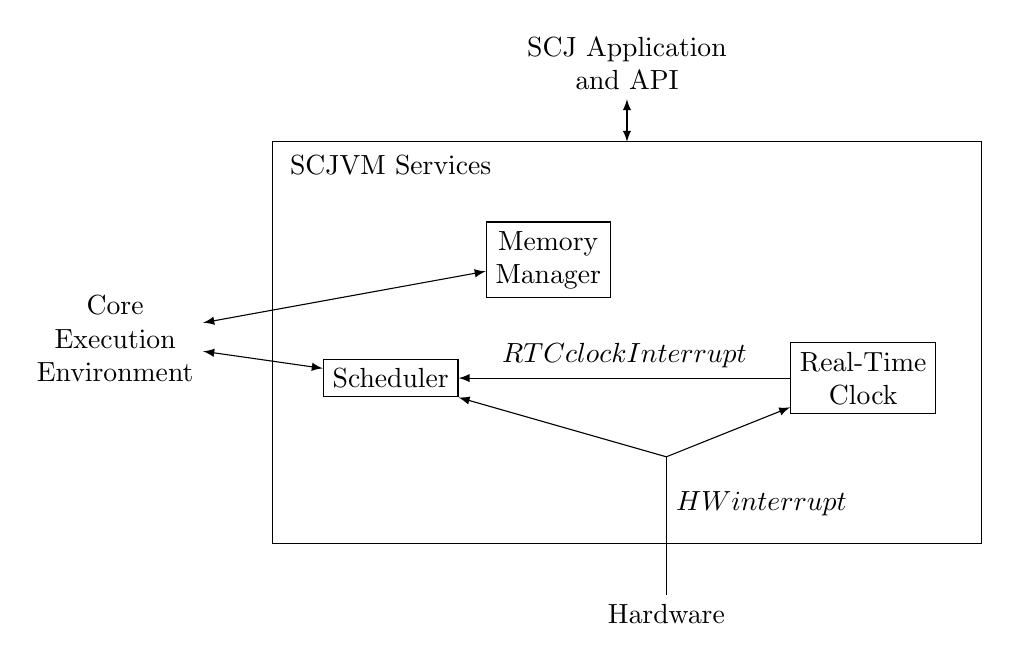
\begin{tikzpicture}
        \node[draw,align=center] (MM)  at (3.5cm,1.5cm) {Memory\\Manager};
        \node[draw,align=center] (S)   at (1.5cm,0cm)  {Scheduler};
        \node[draw,align=center] (RTC) at (7.5cm,0cm)  {Real-Time\\Clock};
        \draw (0cm,-2.1cm) rectangle (9cm,3cm);
        \node at (1.5cm,2.7cm) {SCJVM Services};
        
        \node[align=center] (HW) at (5cm,-3cm) {Hardware};
        
        \draw[-latex] (RTC) edge node[above] {$RTCclockInterrupt$} (S);
        
        \draw[-] (HW) -- node[above right] {$HWinterrupt$} coordinate[pos=1] (X) ++(0cm,2cm);
        \draw[-latex] (X) to (S);
        \draw[-latex] (X) to (RTC);
        
        \node[align=center] (CEE) at (-2cm,0.5cm) {Core\\Execution\\Environment};
        \draw[latex-latex] (S) -- (CEE);
        \draw[latex-latex] (MM) -- (CEE);
        
        \node[align=center] (App) at (4.5cm,4cm) {SCJ Application\\and API};
        \draw[latex-latex] (4.5cm,3cm) -- (App);
      \end{tikzpicture}
      \caption{The structure of the SCJVM services model, showing the
        channels used for communication between the processes in the
        model}
      \label{scjvm-services-model-fig}
\end{figure}